\documentclass[11pt]{article}

%\usepackage{graphicx}
\usepackage[utf8]{inputenc}
\usepackage{wrapfig}
\usepackage[pdftex]{graphicx}

\newcommand{\whitespace}{\rule{\linewidth}{0.0mm}}

\begin{document}
\title{Virtual Reality}
\author{Maximilian Sieß}

%======TITLE PAGE=========
\begin{titlepage}
	\begin{center}
		
\includegraphics[scale=1]{images/uibk} \\
		Leopold-Franzens-Universität Innsbruck
		\linebreak 

		Institute of Computer Science \\
		Interactive Graphics and Simulation Group
		%\maketitle
	
		\whitespace \\[2.0cm]
		\LARGE \textbf{Virtual Reality}\\
		\normalsize Einführung in das Wissenschaftliche Arbeiten\\
		Seminarreport
	
		\whitespace \\[0.8cm]
		Maximilian Sieß
		
		\whitespace \\[2.0cm]
		advised by\\
		Prof. Dr. Matthias Harders
		
		\whitespace \\[4.0cm]
		Innsbruck, \today

	\end{center}
\end{titlepage}

%\newpage 

%=========TABLE OF CONTENTS==============
\tableofcontents

%\section{Abstract}

\newpage
\section{Introduction}
Virtual Reality is the attempt to use technology, such as head mounted display devices, and computer generated graphics, to allow the user to experience a sense of presence in a virtual environment.  This is used in a wide variety of cases, including but not limited to entertainment, education, medical therapy, research, and visualization. Virtual Reality has the potential to fundamentally change the way we experience, and interact with, data and software.

	\section{Definitions}
		\subsection{Virtual Reality}
			Virtual Reality, or VR for short, is the field of computing that aims to create a virtual world, allowing the user to enter, experience and interact with it, by using specific devices to simulate the virtual environment and the feedback it would provide in order to make the experience as real as possible.
			%"Virtual Reality stands for the field of computing which has the objective of creating a virtual world, having one immerse into it and giving one the capability of interacting with this world, while using specific devices to simulate an environment and stimulate one by feedback in order to make the experience as real as possible." 
			\cite{boas13}
			
		\subsection{Immersion}
			Immersion can be differentiated into three different forms. \textit{Engagement}, which has to come from the subject, not the medium. \textit{Engrossment}, which depends on how the software is designed, and is important to affect a subjects emotions, if that is intended. And lastly \textit{total immersion}, or the sense of presence. Total immersion can be understood as what happens when someone is fully engulfed by a piece of media, like a book, movie, or computer game. \cite{Brown:2004:GIG:985921.986048} \\
			Total immersion can also, in the case of VR, be taken more literally as the “extent to which a person's cognitive and perceptual systems are tricked into believing they are somewhere other than their physical location”. \cite{Patrick:2000:ULP:332040.332479} Users of the Oculus Rift have been recorded to be so immersed in the simulation, that they tried to interact with virtual objects by reaching out them them, to for example touch or grab them. \cite{bastiaens14}

		\subsection{Telepresence}
			Telepresence is defined as to have the experience that one is present at another location than his or her physical one.  This name has been coined by Marvin Minsky in the 1980s. \cite{minsky1980telepresence} While Minsky's definition had in mind that ones actions have consequences at another physical location somewhere, which is not necessarily true for VR, Virtual Reality follows the same concept.
			
\section{Related Work}
	\subsection{Technology}
	\subsubsection{Head-Mounted Displays}
	
	\begin{wrapfigure}{r}{0.5\textwidth}
		\vspace{-20pt}
		\begin{center}
			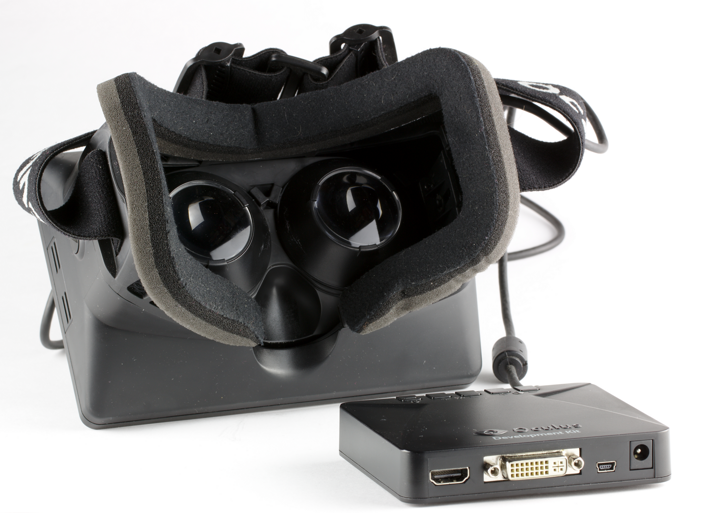
\includegraphics[scale=0.3]{images/or_small.png}
		\end{center}			
		\vspace{-20pt}
			\caption{A Oculus Rift DK1 Headset and HDMI/DVI Converter Box}
		\vspace{-10pt}
	\end{wrapfigure}
	
		Today, the most common form of how Virtual Reality is realized is via head-mounted displays. Goggles with a high density display in it, the same as used in phones. Utilizing special lenses and stereoscopic vision to create a believable view into the virtual environment. \\
		Examples for headsets like these would be the \emph{Oculus Rift} by Oculus VR and one under the working title of \emph{Project Morpheus} by Sony. Both are very similar in execution and produce a VR experience of similar quality. \cite{goradia2014review}
	
	
	At the time of this writing, both have not seen a commercial release, although a development kit for the Oculus Rift is available for purchase.

	\subsubsection{Software}
		Programming software for virtual reality does not differ much from regular computer graphics programming. Most commercial vendors offer their own API that helps translating a virtual camera to a two camera 3D setup. It was found however, that how the camera is used is imperative to not give the user of the virtual reality headset motion sickness or other unpleasant side effects. \cite{seppanen14}
		
		
		For example, moving the camera without the user moving their head has resulted in severely negative feedback from users. The Oculus Rift Best Practices Manual states that "Acceleration creates a mismatch among your visual, vestibular, and proprioceptive senses; minimize the duration and frequency of such conflicts. Make accelerations as short (preferably instantaneous) and infrequent as you can." \cite{yao2014oculus}
	
	\subsubsection{Input Devices}
	With headmounted displays, vision, the groundwork for a feeling of presence in virtual reality, is laid out. Headsets or surround sound systems have been shown to suffice for the audio representation of the virtual environment.\\
	Moving around naturally has proven difficult, however. While video game demos often use a gamepad, it is less than ideal for upholding a sense of presence. Products, such as the XYZ try to enable free movement in virtual reality.
	
	\subsection{Applications of Virtual Reality}
	Most virtual reality hardware developed at this time is geared towards the entertainment business, with a special focus on simulation software, such as flight simulators, and video games, %From Oculus Rift, over Sony's Project Morpheus to Vive by HTC and Valve.
	which can also be used for more humanitarian ways or scientific studies. Games made for these purposes are called \emph{serious games}, and are being used to, for example, allow the user to examine scanned, centuries old manuscripts of which only one copy exists, at a virtual table. \cite{lorenzini2013serious}
	
	Virtual Reality can be used to visualize and teach subjects in ways that were inaccessible before. Teaching history by visiting locations or events of historical importance, for example. \textbf{(Find a paper for that)}
	Another example is 


	%\section{Entertainment}
	%Oculus rift, Valve, Project Morpheus - VIDJA GAMES!
	
	%\section{Education}
	%Look at papers you downloaded
	
	%\section{Therapy}
	%Look at papers or download more!
	
	%\section{Research}
	%Papers!
	
	%\section{Visualization}
	%You know, like for surgery, architecture and stuffs.


\section{Discussion}
With head-mounted displays, headphones and gloves, suspension of disbelief is easier than it ever has been before. All these technologies seem to work to the same goal, to have total immersion without any barriers that make one aware that they are in fact not actually in any virtual space.

And yet this goal still seems very far away.


\section{Conclusion}
I conclude that this paper is bullshit! The End.

\bibliographystyle{plain}
\bibliography{vr_bib}

\section{notes}
Overview of VR - "Virtual Reality development were manly found in the military and academic research until technologies became more cost-effective."
Oh yeah, also input devices are a big factor, shit. Gloves, wands (like the Wii or PS Move) and computer vision.
Also, military wants VR too, woops.
	

arm therapy - Use VR to distract patience from pain while their burn wounds are treated. Seems to work!

unwanted sideeffects - cybersickness or simulator sickness

supply chain eduction - use a VR game to teach

serious games for ancient manuscripts - making vr games about really old books ? Allowing people to experience... reading a really old book.

Todo still:
write more texty text
insert more pictury pictures
polish!
done.

\end{document}
